%!TEX root = ../Main.tex

\chapter{Design}
\section{Design Patterns}
\subsection{State Machine Pattern}
The state machine pattern has been used to develop the system. This is partly done in order to structure the general flow of the algorithm, and partly in order to support concurrent development of the algorithm, as different parts of the algorithm can be implemented simultaneously as different states.

Figure \ref{fig:STM_diagram} shows the state machine diagram for system. It can be seen that the general flow of the system is as follows:
\begin{enumerate}
	\item Set up system.
	\item Create initial population.
	\item Evaluate generation.
	\item If stopping criterion is met, save population and stop. Else-  create new generation, then return to step 3.
\end{enumerate}


\begin{figure}[H]
	\centering
	{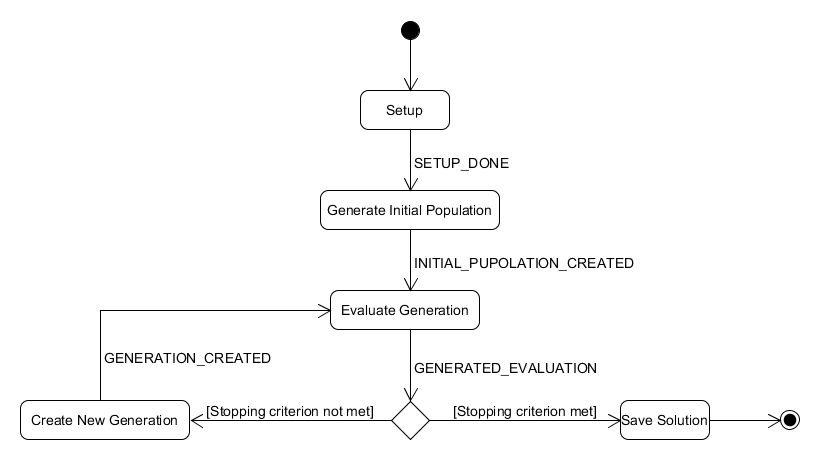
\includegraphics[width=\textwidth]{Images/STM_ROGSAnne.PNG}}\\[0.5cm]
	\caption{State machine diagram for the developed system.}
	\label{fig:STM_diagram}
\end{figure}

To get an overview of the the entire system an activity diagram has been made. This diagram illustrates how the control of the system flows and has a lot in common with the state diagram which is why a lot of the states carries over to this diagram. The activity diagram can be seen on \cref{fig:Activity_diagram}.

\begin{figure}[H]
	\centering
	{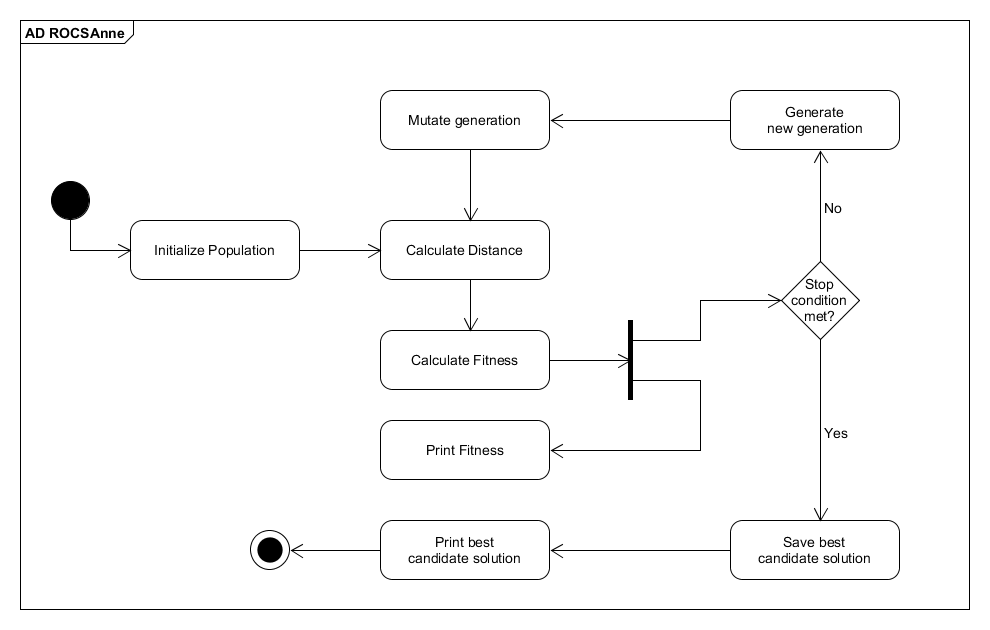
\includegraphics[width=\textwidth]{Images/AD_ROGSAnne.PNG}}\\[0.5cm]
	\caption{State machine diagram for the developed system.}
	\label{fig:Activity_diagram}
\end{figure}



\subsection{Double buffering}
The implemented algorithm operates with two buffers for the population of candidate solutions. The system continuously switches between which buffer is begin used for the old generation and which is being used for the new generation. This is done because the "current" generation must not be altered while a "new" generation is being created. Instead of creating a temporary copy of the "current" generation when creating a new generation, it is faster to have two buffers, one for the "current" generation, and one in which the new generation is being written. When a new generation has been created, the pointer to the new and old generation will change values, letting the newly created generation become the "parent"-generation for a new iteration, and the previously old generation become the target destination for a new generation.

Seeing as the old generation isn't altered during creation of a new generation and that the "target" destination of a newly created sample is known, there are in practice no shared resources, which would ease future implementation of parallelization of the creation of a new generation.

It was considered to use the Command-pattern in order to support parallelization in a future iteration of the project. The idea was to create a Producer-Consumer-pattern, where the creation of samples for a new generation was "ordered" and put in a Command-queue, which several different threads would then "consume" and fill out the buffer. However, each iteration has a known set of "orders" and the "target destination" for the produced samples is known. Assuming that there is a known number of "consumers" that operate equally fast, it would be easier, and as efficient (if not more) to simply assign different threads to create different entries in the new population with predetermined indice. Thus, this idea was deemed unfitting for the purpose of this project.

